\documentclass[UTF8]{ctexart}
\pagestyle{plain}
\usepackage{graphicx}
\usepackage{subfigure}

\title{十一月十号周报}
\date{}

\begin{document}
	本周对git的用法以及上星期所学的部分算法进行总结。git是一个分布式版本控制系统,能够对项目的文件进行集中化的管理,并且具有实时修改、方便回溯、协同工作的诸多优点。其中软件的入门主要看的是廖雪峰的博客,网址:https://www.liaoxuefeng.com/wiki/0013739516305929606dd18
	361248578c67b8067c8c017b000。对于详细步骤就不总结了,就记录一下部分比较重要并且容易忘记的指令及其功能。
	\section{git指令及其功能}
	对于初始化一个git仓库,可以将git bash的当前路径定位到指定路径并用\emph{git init}指令初始化一个git仓库。对于修改完成的文件可以使用\emph{git add (file)}指令添加到暂存区,再通过指令\emph{git commit -m (message)}把修改好的文件添加到分支里。并且可以用指令\emph{git status}可以查看当前分支下的状态,其中包括修改完没提交到暂存区的文件还有没提交到分支的文件,以及分值的文件和当前文件的差别。
	\par
	在写程序过程中难免会发生一些错误,git能够记录每一次提交到分支上的记录,并且会给每次记录一个独有的ID,可以用指令\emph{git log}查看,并用指令\emph{git reset --hard commit-id}回溯到之前的任意版本。
	\par
	而对于多地的控制访问,则需要用到远程仓库,这里用到了远程服务器github。需要在一台机器上获得上传到某github仓库的权限,只需要把电脑的公钥与账号关联起来。而数据用该电脑的私钥加密,这实现了身份认证。
	\par
	要将文件关联一个远程库,即关联到github上的一个repository。使用命令\emph{git remote add origin git@server -name:path/repo-name.git}。关联以后可以通过指令\emph{git push -u origin master}来第一次推送当前目录master分支下的所有内容。此后每次本地修改后,就可以用\emph{git push origin master}推送更新。
	\par
	如果在另一台电脑需要复制相同的工作环境,则可以用命令\emph{git clone git@server -name:path/repo-name.git}克隆出一个提交的库。如果要载入更新,则可以用\emph{git pull}抓取更新。
	\section{动态规划算法}
	动态规划的第一个问题是钢条切割利益最大化的问题,由两种方式可以解决此问题,第一种是自顶向下的方法,另一种是自底向上的方法。
	\begin{figure}[h]
		\centering
		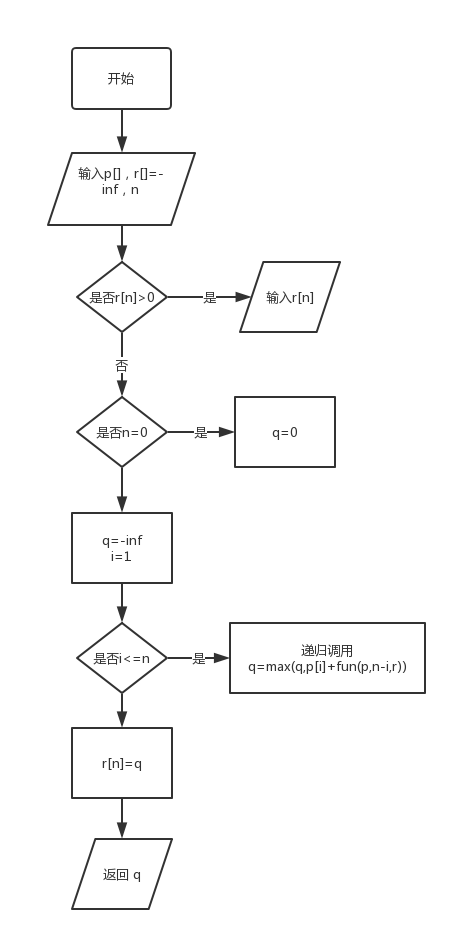
\includegraphics[width=10cm,height=13cm]{1}
		\caption{带备忘的自顶向下法}
	\end{figure}
	\par
	相比较而言,自底向上的算法更加简单而且效率更高。其算法流程图如下。
	\begin{figure}[h]
		\centering
		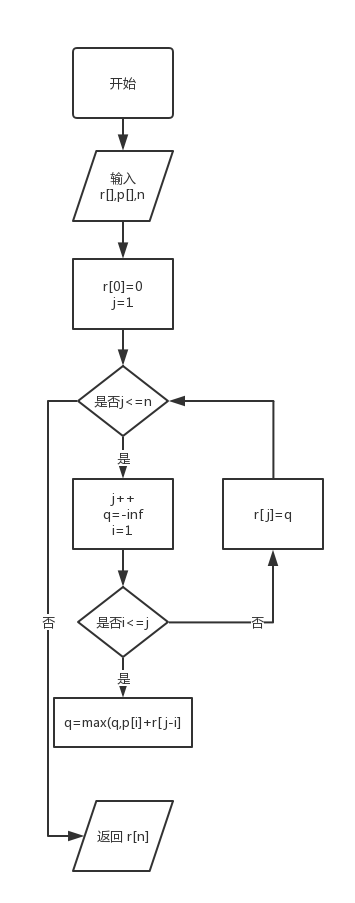
\includegraphics[width=7cm,height=12cm]{2}
		\caption{自底向上的方法}
	\end{figure}
	\par
	而对于矩阵链乘法则是另一个经典的动态规划问题,通过改变一串矩阵相乘的顺序可以大大减少计算量。通过此算法可以得到最优的相乘结果。
	\begin{figure}[h]
		\centering
		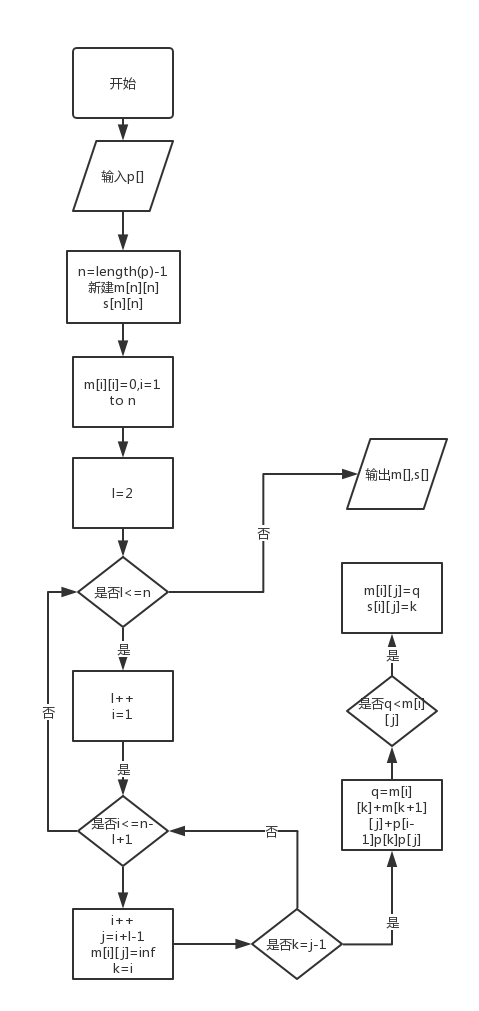
\includegraphics[width=7cm,height=15cm]{3}
		\caption{矩阵相乘最优化算法}
	\end{figure}
	\par
	将这几个算法写成了C++函数的形式,方便调用。具体的代码另附文件。
\end{document}